\documentclass[10pt,a4paper]{article}

\usepackage{polski}
\usepackage[utf8]{inputenc}
\usepackage[polish]{babel}
\usepackage{hhline}
\usepackage{pgfplots}
\usepackage{multicol}
%\usepackage{slashbox}
\usepackage{graphicx}
\usepackage{caption}
\usepackage{subcaption}
\usepackage{colortbl}
\usepackage{geometry}
\usepackage{listings}
\geometry{a4paper, total={170mm,257mm}, left=20mm, top=20mm }
\lstset
{
    language=C++,
    basicstyle=\footnotesize,
    numbers=left,
    stepnumber=1,
    showstringspaces=false,
    tabsize=1,
    breaklines=true,
    breakatwhitespace=false,
}
\author{Sebastian Maciejewski 132275 i Jan Techner 132332\\
grupa I1, zajęcia we wtorki o 15:10, tygodnie nieparzyste,\\
email: maciejewski.torun@gmail.com}
\title{Porównywanie efektywności metod mnożenia macierzy}
\date{30 kwietnia 2019}
\setlength{\parindent}{0pt}
\newcommand{\forceindent}{\leavevmode{\parindent=3em\indent}}
\begin{document}
\maketitle
\section{Wstęp}
Sprawozdanie dotyczy zadania w wariancie 22. - porównywanie efektywności metod
mnożenia macierzy:\\
- dla 3 pętli kolejność jki, podział pracy przed 1. pętlą\\
- dla 6 pętli kolejność pętli zewnętrznych ijk, wewnętrznych iijjkk,
podział pracy przed 4. pętlą\\
\\
Wszystkie pomiary zostały wykonane na komputerach laboratoryjnych w sali 2.7.6.
\section{Analiza przygotowania eksperymentu}
\subsection{Kod wykorzystywany przy pomiarach}
Kod, którego używaliśmy w eksperymencie został tak podzielony, aby cała
logika przetwarzania znajdowała się w pojedynczej funkcji. Poniżej prezentowany
jest kod tylko tych funkcji - generowanie macierzy i wypełnianie jej
losowymi liczbami, liczenie czasu i wypisywanie wyników działają w ten
sam sposób dla wsystkich wariantów przetwarzania.
\subsubsection{Metoda 3 pętli - równolegle}
\begin{lstlisting}
    void multiply_matrices_JKI()
    {
    #pragma omp parallel for 
        for (int j = 0; j < COLUMNS; j++)
            for (int k = 0; k < COLUMNS; k++)
                for (int i = 0; i < ROWS; i++)
                    matrix_r[i][j] += matrix_a[i][k] * matrix_b[k][j];
    }
\end{lstlisting}

\subsubsection{Metoda 3 pętli - sekwencyjnie}
\begin{lstlisting}
    void multiply_matrices_IKJ_sequentially() 
    {
        for (int i = 0; i < ROWS; i++)
            for (int k = 0; k < COLUMNS; k++)   
                for (int j = 0; j < COLUMNS; j++)
                    matrix_r[i][j] += matrix_a[i][k] * matrix_b[k][j];
    }
\end{lstlisting}

\subsubsection{Metoda 6 pętli - równolegle}
\begin{lstlisting}
    void multiply_matrices_IJK_IIJJKK()
    {
        int r = 10;
        for (int i = 0; i < ROWS; i += r)
            for (int j = 0; j < COLUMNS; j += r)
                for (int k = 0; k < COLUMNS; k += r)
    #pragma omp parallel for
                    for (int ii = i; ii < i + r; ii++)
                        for (int jj = j; jj < j + r; jj++)
                            for (int kk = k; kk < k + r; kk++)
                                matrix_r[ii][jj] += matrix_a[ii][kk] * matrix_b[kk][jj];
    }
\end{lstlisting}
\newpage

\subsection{Analiza podziału pracy na wątki}
\subsubsection{Dyrektywy OpenMP}
W naszym kodzie używamy dyrektyw 'pragma omp parallel for', które sprawiają, że iteracje pętli
będą wykonane w sposób równoległy przez kilka wątków. Każdy z wątków wykona jednakowy zakres
iteracji, w naszym wypadku, przy podziale na 4 wątki, pierwszy wątek wykona pierwszą $\frac{1}{4}$
operacji, drugi kolejną itd. Dopiero po zakończeniu przetwarzania przez wszystkie wątki następuje
synchronizacja i przejście dalej - do zakończenia pomiaru czasu.

\subsubsection{Analiza ryzyka wystąpienia wyścigu i zjawiska false sharingu}
Zjawisko wyścigu, czyli równoległa modyfikacja tej samej zmiennej przez różne procesy, nie
występuje w naszym kodzie.\\
Aby się o tym przekonać wystarczy zwrócić na to, że w naszym przypadku,
w równoległym przetwarzaniu dla 3 pętli mamy zapis do $matrix\_r[i][j]$, gdzie wartości $j$ są
dzielone pomiędzy procesy z powodu wystąpienia dyrektywy 'parallel for' przed pętlą odpowiedzialną
za inkrementację licznika kolumn $j$ (2.1.1, linijki od 3 do 7). Co za tym idzie każdy proces zawsze zapisuje do innej kolumny
niż pozostałe, więc zjawisko wyścigu nie występuje w tym przypadku.\\
Podobna sytuacja występuje przy 6 pętlach - każdy proces zapisuje do osobnego wiersza z powodu
wystąpienia dyrektywy 'parallel for' przed pętlą odpowiedzialną za inkrementację zmiennej $ii$
(2.1.3, linijki od 7 do 11) - w tym przypadku również nie dojdzie do wyścigu.\\
\\
Inaczej sytuacja ma się w przypadku zjawiska false sharingu. False sharing występuje wtedy, gdy
różne procesy zapisują zmienne znajdujące się w tej samej linii pamięci - wówczas kopie linii
w pamięciach podręcznych innych procesów stają się nieaktualne i dany proces musi ponownie pobrać
linię z pamięci aby zapewnić spójność pamięci podręcznej. To zajmuje czas, więc takie zjawisko
jest nieporządane, gdyż wpływa negatywnie na efektywność przetwarzania.\\
Długość linii pamięci w systemach, na których wykonywane były pomiary to 64B, zatem w każdej
linii pamięci mieści się 16 zmiennych typu float, używanych prez nas w obliczeniach. Rozmiary
instancji w naszych pomiarach były $\geq 400$. Mając to na uwadze, możemy się zająć analizą ryzyka
wystąpienia zjawiska false sharingu.\\
W wersji przetwarzania równolegle dla 3 pętli mamy do czynienia z podziałem pracy przed 1. pętlą, $j$,
która odpowiada da licznik kolumn.\\
DUŻY ZNAK ZAPYTANIA ? NAD TYM:\\
W tym wypadku możemy stwierdzić, że z uwagi na to, iż każdy z procesów zapisuje dane
jedynie do swojej kolumny macierzy, zjawisko false sharingu nie wystąpi gdyż rozmiar jednej kolumny jest
znacznie większy od rozmiaru jednej linii pamięci - dla instancji o wielkości 400, w kolumnie
mieści się około 50 linii pamięci. Jedynym miejscem, w którym to zjawisko może wystapić są brzegi
kolumn. (ALE CHYBA JEDNAK WIERSZY)\\
CZY JEDNAK WYSTĄPI BO MACIERZ JEST UŁOŻONA W PAMIĘCI WIERSZAMI I KAŻDY PROCES ROBI SOBIE KOPIĘ
WIERSZA, WIĘC JAK KTOŚ COŚ ZMIENI W INNEJ KOLUMNIE TO POTRZEBNY JEST PONOWNY ODCZYT CAŁEGO WIERSZA?\\
\\
DO OBGADANIA, BO JEŚLI JEST TAK Z WIERSZAMI, TO W 6 PĘTLACH NIE BĘDZIE FALSE SHARINGU A W 3 BĘDZIE.
\\

\newpage

\subsubsection{Podział przetwarzania w metodzie 3-pętlowej}
\begin{figure}[h]
    \centering
    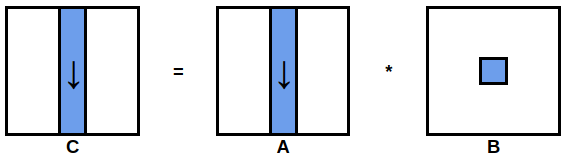
\includegraphics[width=0.5\textwidth]{3loops1.png}
    \caption{Obszar danych dla jednej wewnętrznej pętli}
\end{figure}

JAKIŚ OPIS

\begin{figure}[h]
    \centering
    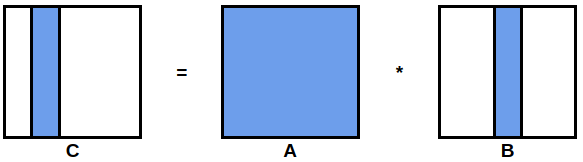
\includegraphics[width=0.5\textwidth]{3loops2.png}
    \caption{Obszar danych dla dwóch wewnętrznych pętli}
\end{figure}
JAKIŚ OPIS

\newpage

\subsubsection{Podział przetwarzania w metodzie 6-pętlowej}
TODO OPISY

\begin{figure}[h]
    \centering
    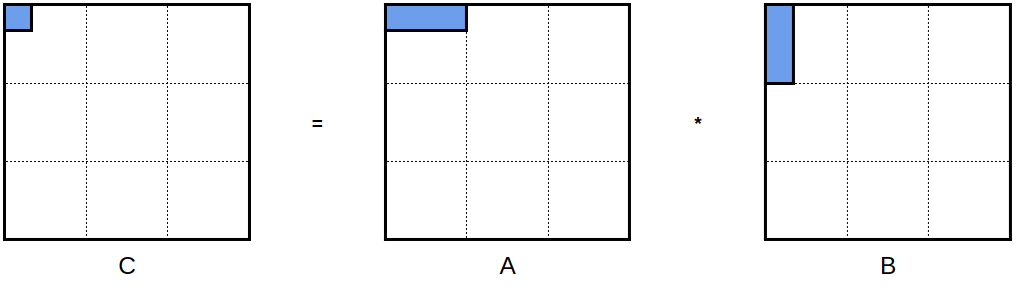
\includegraphics[width=0.5\textwidth]{6loops1.png}
    \caption{Obszar danych dla pętli $kk$}
\end{figure}

\begin{figure}[h]
    \centering
    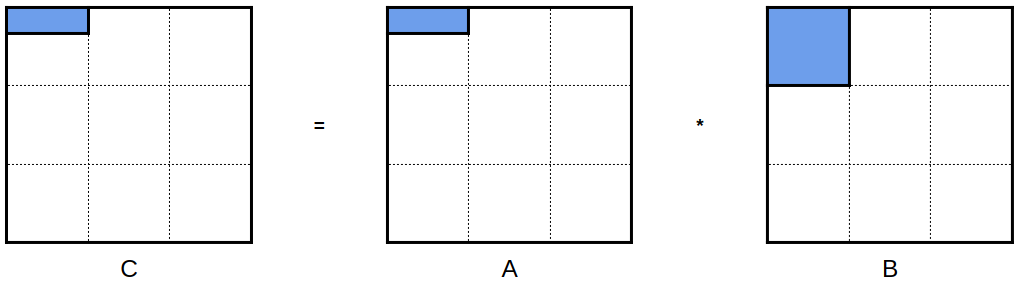
\includegraphics[width=0.5\textwidth]{6loops2.png}
    \caption{Obszar danych dla pętli $jj$, $kk$}
\end{figure}

\begin{figure}[h]
    \centering
    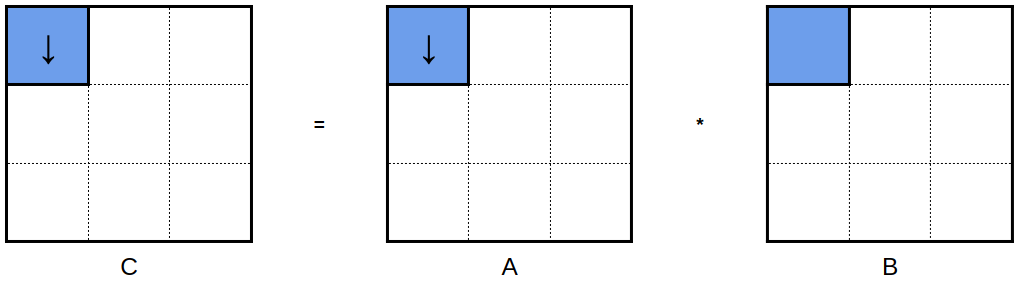
\includegraphics[width=0.5\textwidth]{6loops3.png}
    \caption{Obszar danych dla pętli $ii$, $jj$, $kk$}
\end{figure}

\newpage

\subsection{Analiza lokalności czasowej}
Znaczącym czynnikiem mającym wpływ na efektywność przetwarzania jest czas dostępu do
danych. Ten czas jest znacznie krótszy przy dostępie podręczniej pamięci procesora niż
przy konieczności odwołania się do pamięci RAM. Bardzo ograniczona pojemność pamięci
podręcznej sprawia, że kod powinien być pisany w taki sposób, aby maksymalizować
wykorzystanie danych już załadowancyh do pamięci podręcznej i minimalizować ilość
odczytów z RAM. Przetwarzanie jest efektywne wtedy, gdy kod charakteryzuje się
czasową lokalnością odwołań do pamięci, czyli wielokrotnym wykorzystaniem danych załadowanych
do pamięci podręcznej zanim zostaną zastąpione innymi danymi odczytanymi z RAM.\\
Zakładamy, że rozmiar pamięci podręcznej procesora, na którym przeprowadzane są
obliczenia to 6 MB. Jest to pojemność pamięci L3 - L2 nie jest tu brane pod uwagę,
ponieważ część danych obecnych w niej pokrywa się z danymi w L3. Również pamięć L1
jest przy tym założeniu pomijana, ponieważ jej pojemność jest tak mała, że jej uwzględnianie
nie miało by znaczącego wpływu na obliczane wielkośći instancji.\\
Przy obliczeniach zakładamy, że 1 MB = 1000 KB = 1000000 B, przy czym pojedyncza zmienna typu
float, z których korzystamy, ma rozmiar 4 B.
\\
Dla metody 3 pętli wzór, którego używamy do obliczania rozmiaru instancji, dla której
będzie zachowana lokalność czasowa to:
$$
    n^2 * 4 + n * 16 * 4 + n * 16 * 4 \leq \frac{6 * 1000000}{4}
$$
przy czym $n$ to rozmiar instancji.\\
Wzór ma taką postać, bo DLACZEGO DOKŁADNIE TAK BYŁO?\\
Po obliczeniu uzyskana wartość $n$ rozmiaru instancji, dla której wciąż będzie zachowana
lokalność czasowa to w przybliżeniu $n \leq 596$.\\
Dla metody 6 pętli wzór do obliczenia rozmiaru instancji ma postać:
$$
    3*4*r^2 \leq 6000000
$$
gdzie $r$ to rozmiar wykorzystywanego bloku, pobieranego każdorazowo z macierzy.\\
Wzór ma taką postać ponieważ DLACZEGO DOKŁADNIE\\
Po obliczeniu wartość $r$, dla której będzie zachowana lokalność czasowa to $r \leq 707$.

\subsection{Analiza lokalności przestrzennej}
Lokalność przestrzenna jest związana z występowaniem w systemie pamięci wirtualnej.
Jest mechanizm, który umożliwia procesowi pracę w jednym, ciągłym obszarze pamięci operacyjnej,
nawet gdy fizycznie jest ona pofragmentowana lub część z niej znajduje się w pliku wymiany,
który procesy mogą wykorzystać jako dodatkową pamięć w przypadku, gdy w systemie brakuje
fizycznej pamięci operacyjnej. Pamięć wirtualna niesie ze sobą pewne konsekwencje -
najważniejszą z nich jest to, że teraz procesy muszą posługiwać się adresami logicznymi
zamiast fizycznymi adresami mającymi bezpośrednie odwzorowanie w pamięci RAM.
Taka pamięć jest dzielona na strony o rozmiarze 4 kB, które stanowią jeden, ciągły obszar w pamięci.
Aby taki system mógł działać, pamięć RAM jest dzielona na ramki, których rozmiar odpowiada
rozmiarowi stron. Strony mogą się znajdować w pamięci lub we wspomnianym wyżej pliku wymiany,
co sprawia, że procesor musi posługiwać się logicznymi adresami aby uzyskać dostęp do danych.//
Taka organizacja pamięci wymusza obecność mechanizmu tłumaczenia adresów logicznych
na fizyczne, czyli odwzorowania adresów strony na adres ramki pamięci. Informacje o takich
odwzorowaniach znajdują się w tablicy stron. W tym miejscu stosuje się pewne usprawnienie, jako, że
przeglądanie takiej tablicy przy każdym odwołaniu byłoby bardzo mało wydajne. Tym usprawnieniem
jest bufor translacji adresu TLB, który posiada określoną, stałą liczbę adresów stron i odpowiadającyh
im ramek, dzięki czemu można szybko dokonać translacji adresu logicznego na fizyczny.
Jednak tak jak w pamięci podręcznej, tak i w buforze translacji występuje ograniczenie rozmiaru.\\
\\
Program chechuje się zachowaniem lokalności przestrzennej wtedy, kiedy nie występują sytuacje,
w których w buforze translacji nie znajduje się adres szukanej strony. W procesorze, z którego
korzystaliśmy przy obliczeniach bufor translacji mieści 544 pary adres strony - adres ramki.
Każda ze stron pamięci wirtualnej ma rozmiar 4 kB, tak więc mieści 1024 liczby z wykorzystywanej
przez nas macierzy.


Aby znaleźć wielkośći instancji, dla których przetwarzanie zachowa lokalność przestrzenną dla
3 pętli posłużyliśmy się wzorem:
$$
    \frac{n*n}{1024} + n + n \leq 544
$$
gdzie $n$ to rozmiar instancji.\\
Taka postać wzoru wynika z Z CZEGO ?\\
\\
Po obliczeniu wartość $n$, dla której będzie zachowana lokalność przestrzenna to $n \leq 243$.
\\

Dla 6 pętli wzór na znalezienie takich wartośći $n$ i $r$, dla których przetwarzanie zachowa
lokalność przestrzenną, wygląda następująco:
$$
    min\Big(r, \frac{r*n}{1024}\Big) + 2*min\Big(\frac{r}{4}, \frac{\frac{r}{4} * n}{1024}\Big) \leq 544
$$
gdzie $n$ to rozmiar instancji, a $r$ to rozmiar wykorzystywanego bloku.\\
Wzór ma taką postać ponieważ DLACZEGO ? \\ I JAK OPISAĆ OBLICZANIE WARTOŚCI TEJ FUNKCJI 2 ZMIENNYCH
\\
\section{Analiza wyników eksperymentu pomiarowego}
\subsection{Wstępny opis eksperymentu pomiarowego}
Eksperyment został przeprowadzony na komputerach w sali laboratoryjnej 2.7.6 przy
wykorzystaniu funkcji opisanych w punkcie 2.1 wywoływanych w programie, którego jedynym
zadaniem poza wywołaniem wymienionych wyżej funkcji było losowanie macierzy
(na początku, przed rozpocżeciem pomiaru czasu) i mierzenie czasu przetwarzania
(na podstawie stanu zegara przed i po wywołaniu funkcji). Po podaniu wielkości instancji
i kompilacji programu poddawaliśmy go analizie w programie CodeXL. Ogólnie mierzone (lub dane)
były następujące wartości:
\begin{center}
    \begin{tabular}{ |c|c|c| }
        \hline
        Zmienna & Oznaczenie & Wartość progu \\
        \hline
        Wielkość instancji & n &  \\
        Wielkość okna & r &  \\
        Czas przetwarzania & Tobl &  \\
        Liczba instrukcji assemblera & LIA &  250 000\\
        Liczba cykli procesora & LCP & 250 000 \\
        Liczba dostępów do L1 & LDP & 250 000 \\
        Liczba braków trafień do L3 & BTL3 & 50 000 \\
        Liczba braków trafień do bufora translacji & BTBT & 50 000 \\
        \hline
    \end{tabular}
    \captionof{table}{Oznaczenia i progi zmiennych}
\end{center}
Wielkością instancji określamy rozmiar mnożonej macierzy kwadratowej.\\
Pomiary zbierane były w taki sposób, aby nie uruchamiać na raz analizy zbyt wielu
parametrów, gdyż mogłoby to zakłócić wyniki. Aby tego uniknąć mierzyliśmy najpierw 
LDP, BTL3 i BTBT, a dopiero później LIA i LCP. Odczytane wyniki zapisywaliśmy do 
załączonego arkusza kalkulacyjnego. Dokonaliśmy też wstępnej analizy instrukcji
assemblera, które składały się na nasz program aby zobaczyć które z nich najbardziej
obciążały procesor (było ich najwięcej).
\subsection{Wyniki uzyskane w eksperymencie}
\begin{center}
    \begin{tabular}{ |c|c|c|c|c|c|c|c| }
        \hline
        n & Tobl & LIA & LCP & LDP & BTL3 & BTBT \\
        \hline
        400	& 0.078	& 1413 & 1871 & 925 & 35 & 1\\
        \hline
        450	& 0.109 & 1980 & 4914 &	1329 & 53 &	16\\
        \hline
        550	& 0.289 & 3566 & 15405 & 2370 &	113	& 1036\\
        \hline
        600 & 0.625 & 4554 & 29754 & 3159 &	136 & 2697\\
        \hline
        700	& 1.683 & 6856 & 77515 & 4999 & 349	& 7458\\
        \hline
    \end{tabular}
    \captionof{table}{Wyniki dla 3 pętli, przetwarzanie równolegle}
\end{center}

\begin{center}
    \begin{tabular}{ |c|c|c|c|c|c|c|c|c| }
        \hline
        n & r & Tobl & LIA & LCP & LDP & BTL3 & BTBT \\
        \hline
        1500 & 100 & 1.5780 & 233901 & 97207 & 33332 & 2688 & 44\\
        \hline
        1500 & 300 & 2.6770 & 105947 & 131667 &	33506 & 2002 & 153\\
        \hline
        1500 & 400 & 4.4530 & 98107 & 232887 & 87960 & 1192 & 653\\
        \hline
        1500 & 500 & 2.9530 & 241691 & 154389 &	31834 & 720 & 7617\\
        \hline
        1500 & 750 & 7.3280 & 101394 & 366565 &	31171 & 1086 & 40351\\
        \hline
        2000 & 200 & 3.6700 & 242986 & 204930 &	74343 & 2825 & 69\\
        \hline
    \end{tabular}
    \captionof{table}{Wyniki dla 6 pętli, przetwarzanie równolegle}
\end{center}

\begin{center}
    \begin{tabular}{ |c|c|c|c|c|c|c|c| }
        \hline
        n & Tobl & LIA & LCP & LDP & BTL3 & BTBT \\
        \hline
        400	& 0.0310 & 774 & 582 & 375 & 18 & 1\\
        \hline
        450	& 0.0630 & 1073 & 832 &	602 & 17 & 1\\
        \hline
        550	& 0.0940 & 1877 & 1431 & 1060 & 24 & 1\\
        \hline
        600	& 0.0940 & 2329 & 1577 & 1097 &	23 & 0\\
        \hline
        700	 & 0.1660 &	3616 & 2441 & 1685 & 42 & 3\\
        \hline
        800	& 0.2340 & 5299 & 3534 & 2454 &	42 & 8\\
        \hline
    \end{tabular}
    \captionof{table}{Wyniki dla 3 pętli, przetwarzanie sekwencyjne}
\end{center}

\end{document}